% T_F := SL2(Z).T cap F = { tau in F : Im tau <= 1 }, i.e. all of T carried into
% the standard fundamental domain.  Poles here are not excluded; they are the
% ones for which the correction Q_f of Lemma 4.26 is needed.
%
% Bounded below by |tau| = 1 and above by Im tau = 1; hyperbolic area pi/3 - 1
% = (pi-3)/3 = area(T)/3, the 3 being the order of U, which rotates T about its
% interior fixed point rho+1.
%
% Compile standalone:   pdflatex TF_region.tex
\documentclass[border=8pt]{standalone}
\usepackage{lmodern}
\usepackage{amsmath,amssymb}
\usepackage{tikz}
\usetikzlibrary{arrows.meta}

\definecolor{Ffill}{HTML}{DCE7F2}\definecolor{Fline}{HTML}{7F9AB4}
\definecolor{Tfill}{HTML}{F0A860}\definecolor{Tline}{HTML}{A8410A}
\definecolor{Gline}{HTML}{1F4E79}

\begin{document}
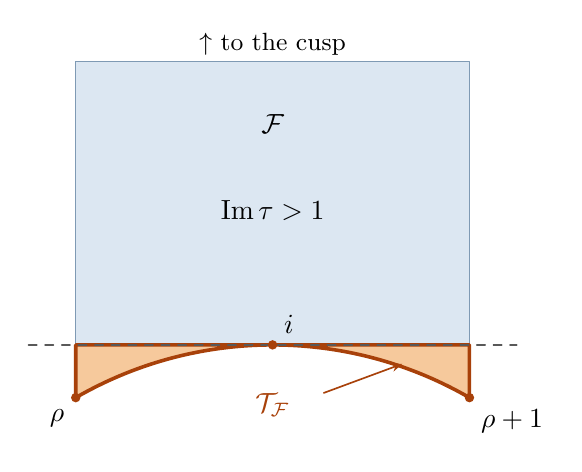
\begin{tikzpicture}[scale=5,line join=round,line cap=round]
\def\ytop{1.72}
\def\rh{0.86602540378}

% ---- the part of F above the contour: poles here are allowed ----
\fill[Ffill,draw=Fline,line width=0.5pt]
  (-0.5,1) -- (-0.5,\ytop) -- (0.5,\ytop) -- (0.5,1) -- cycle;

% ---- T_F: the part of F at or below the contour ----
\fill[Tfill,opacity=0.62]
  (-0.5,\rh) -- (-0.5,1) -- (0.5,1) -- (0.5,\rh)
  arc[start angle=60, end angle=120, radius=1] -- cycle;
\draw[Tline,line width=1.3pt]
  (-0.5,\rh) -- (-0.5,1) -- (0.5,1) -- (0.5,\rh)
  arc[start angle=60, end angle=120, radius=1] -- cycle;

% ---- the contour height ----
\draw[dashed,gray!70!black,line width=0.6pt] (-0.62,1) -- (0.62,1);

% ---- annotations ----
\node[anchor=south,inner sep=2pt] at (0,1.30) {${\rm Im}\,\tau>1$};
\node[anchor=north,inner sep=1pt,Tline] at (0,0.885) {$\mathcal{T}_{\mathcal{F}}$};
\draw[Tline,line width=0.6pt,-{Stealth[length=4pt]}] (0.13,0.878) -- (0.33,0.952);
\node at (0,1.56) {$\mathcal{F}$};
\node[anchor=south,inner sep=2pt,font=\small] at (0,\ytop) {$\uparrow$ to the cusp};

% ---- marked points ----
\foreach \x/\y/\l/\a in {0/1/{i}/{south west}, -0.5/\rh/{\rho}/{north east},
                         0.5/\rh/{\rho+1}/{north west}}{
  \fill[Tline] (\x,\y) circle[radius=0.012];
  \node[anchor=\a,inner sep=4pt] at (\x,\y) {$\l$};}
\end{tikzpicture}
\end{document}
